\documentclass[a4paper,11pt]{report}

\usepackage[utf8]{inputenc}
\usepackage[T1]{fontenc}
\usepackage[french]{babel}
\usepackage{amsmath,amssymb}
\usepackage{graphicx}
\graphicspath{{./}{./notebooks/figures/}{./cas_4/}{./cas_1_2/}{./cas_3/}{./traitement_donnees/}{./revue_litterature/}}
\usepackage{booktabs}
\usepackage{tabularx}
\usepackage[hidelinks]{hyperref}
\usepackage{enumitem}
% interligne
\usepackage{setspace}
\onehalfspacing

% COULEUR (xcolor requis pour gray!10 utilisé par listings)
\usepackage{xcolor}
\definecolor{Valentia}{RGB}{233,78,82}
\definecolor{Titleblue}{RGB}{0, 0, 255}

\usepackage{geometry}
\geometry{margin=2.5cm, headheight=14pt}

% En-tête et pied de page sur toutes les pages
\usepackage{fancyhdr}
\pagestyle{fancy}
\fancyhf{}
\fancyhead[L]{\textit{Architecture des Systèmes Intelligents}}
\fancyhead[R]{\textit{Combinaison de classeurs, explicabilité des modèles}}
\renewcommand{\headrulewidth}{0.4pt}
\fancyfoot[L]{Université De Dschang}
\fancyfoot[C]{\thepage}
\fancyfoot[R]{2025 - 2026}
\fancypagestyle{plain}{%
  \fancyhf{}
  \fancyhead[L]{\textit{Architecture des Systèmes Intelligents}}
  \fancyhead[R]{\textit{Combinaison de classeurs, explicabilité des modèles}}
  \renewcommand{\headrulewidth}{0.4pt}
  \fancyfoot[L]{Université De Dschang}
  \fancyfoot[C]{\thepage}
  \fancyfoot[R]{2025 - 2026}
}

\usepackage{float}

\usepackage{listings}
\usepackage{listingsutf8}
\lstset{inputencoding=utf8,basicstyle=\ttfamily,breaklines=true,backgroundcolor=\color{gray!10}}
\lstdefinestyle{reportPython}{language=Python, frame=single, breaklines=true, basicstyle=\ttfamily\small}
% Packages algorithm/algpseudocode désactivés si non installés (texlive-science).
% Décommenter si besoin d'écrire des algorithmes :
% \usepackage{algorithm}
% \usepackage{algpseudocode}
% \algnewcommand\algorithmicforeach{\textbf{pour chaque}}
% \algdef{S}[FOR]{ForEach}[1]{\algorithmicforeach\ #1\ \textbf{faire}}

% Numérotation des sections en 1, 2, 3 (sans chapitre)
\renewcommand{\thesection}{\arabic{section}}
\numberwithin{figure}{section}
\numberwithin{table}{section}

% Espacement des titres (sections)
\usepackage{titlesec}
\titlespacing*{\section}{0pt}{2.5ex plus .2ex}{1.5ex plus .2ex}
\titlespacing*{\subsection}{0pt}{2ex plus .2ex}{1ex plus .2ex}
\titlespacing*{\subsubsection}{0pt}{1.5ex plus .2ex}{0.8ex plus .2ex}

% Profondeur de la table des matières
\setcounter{tocdepth}{3}

% Indentation et listes
\setlength{\parindent}{1.5em}
\setlist{leftmargin=*, itemsep=2pt}

% Environnements partagés (parties 2 et 3)
\newenvironment{definition}[1]{\par\medskip\paragraph{Définition (#1).}\leavevmode\noindent}{\par\medskip}
\newenvironment{pointcle}{\par\medskip\paragraph{Point clé.}\leavevmode\noindent}{\par\medskip}
\newenvironment{attention}{\par\medskip\paragraph{Attention.}\leavevmode\noindent}{\par\medskip}
\newenvironment{exemple}[1]{\par\medskip\paragraph{Exemple (#1).}\leavevmode\noindent}{\par\medskip}

\newcommand{\HRule}{\rule{\linewidth}{0.5mm}}

\title{Combinaison de classeurs, explicabilité des modèles}
\author{DNJOMOU YONMBA WILFRIED LOIC  \\
KENFACK LEONEL \\
SAGUEU WAKAM DILANE \\
NZOGNING MBONDA SOCRATE \\}
\date{Mars 2025}

\begin{document}
\widowpenalty=3000
\clubpenalty=3000

\begin{titlepage}
    \thispagestyle{empty}
    \centering
    
\includegraphics[width=\textwidth]{entete.png}\\[2.0cm]

    \textsc{Architecture des Systèmes Intelligents}\\[0.5cm]

    % Titre principal
    \HRule \\[0.4cm]
    \color{Titleblue}
    \fontsize{20}{23.4}\selectfont
    \huge \bfseries Travaux Pratiques: Combinaison de classeurs, explicabilité des modèles \\[0.4cm]
    \color{black}

    \HRule \\[0.4cm]


    \vspace{2cm}

    % Présenté par
    \fontsize{15}{18}\selectfont
    \color{black}
    \textbf{Présenté par :}\\[0.5cm]

    \begin{tabular}{l l}
        \textbf{DNJOMOU YONMBA WILFRIED LOIC} & \textbf{CM-UDS-24SCI0999} \\
        \textbf{KENFACK LEONEL} & \textbf{CM-UDS-17SCI0998} \\
        \textbf{SAGUEU WAKAM DILANE} & \textbf{CM-UDS-24SCI1040} \\
        \textbf{NZOGNING MBONDA SOCRATE} & \textbf{CM-UDS-19SCI2910} \\
    \end{tabular}

    \vspace{1cm}

    % SUPERVISEUR
    \fontsize{15}{18}\selectfont
    \color{black}
    \textbf{Superviseur :} Pr. KENGNE TCHENDJI Vianney\\[0.5cm]

    \vfill

    \hrulefill

    \vspace{5mm}

    \centering{\large{\bf Année académique 2025-2026 }}
\end{titlepage}

\tableofcontents
\listoffigures
\listoftables
\newpage

% Introduction
\newpage
\section{État de l'art}
\label{sec:etat-art}

Cette section présente cinq articles consacrés à la prédiction de la maladie rénale chronique par apprentissage automatique. Chaque article est résumé ci-dessous~; le tableau~\ref{tab:ckd-articles} en donne une vue synthétique.

\paragraph{Almansour et al. (2022) \cite{almansour2022ckd}.}
Les auteurs comparent la forêt aléatoire, la machine à vecteurs de support et l'arbre de décision pour la prédiction et le staging de la maladie rénale chronique. La sélection de variables repose sur l'analyse de variance et l'élimination récursive des variables avec validation croisée. La forêt aléatoire avec élimination récursive surpasse la machine à vecteurs de support et l'arbre. L'étude souligne l'importance d'une détection précoce des stades de maladie rénale chronique pour limiter les complications (hypertension, anémie, troubles minéraux, etc.). Publication dans \emph{Journal of Big Data}.

\paragraph{Swapna et Chandra (2021) \cite{swapna2021ckd}.}
Sur le jeu UCI maladie rénale chronique (400 observations, 25 paramètres), les auteurs combinent la forêt aléatoire et AdaBoost via un classifieur à vote. Le prétraitement inclut l'imputation des valeurs manquantes (en tenant compte de l'asymétrie) et une sélection de variables par corrélation. Le modèle hybride atteint jusqu'à 100\,\% d'exactitude selon les sous-ensembles de variables, avec validation sur plusieurs métriques (exactitude, précision, rappel, F1). Publication dans \emph{EAI Endorsed Transactions on Pervasive Health and Technology}.

\paragraph{Swain et al. (2023) \cite{swain2023ckd}.}
Les auteurs construisent un classifieur de maladie rénale chronique à partir de jeux publics en appliquant une imputation des manquants, un équilibrage des classes par surotéchantillonnage et une mise à l'échelle, puis une sélection de variables par test du Chi-carré. La machine à vecteurs de support et la forêt aléatoire sont comparées en validation croisée 10 folds~: la machine à vecteurs de support obtient la meilleure exactitude (99,33\,\%), devant la forêt aléatoire (98,67\,\%). L'objectif est de réduire l'incertitude clinique en automatisant l'analyse des marqueurs. Publication dans \emph{Electronics}.

\paragraph{Singh et al. (2024) \cite{ckd_xai_nature2024}.}
Sur 491 patients (56 avec maladie rénale chronique, 435 sans), cinq modèles sont évalués (régression logistique, forêt aléatoire, arbre, Naïve Bayes, XGBoost) et expliqués par les méthodes SHAP et LIME. XGBoost obtient la meilleure performance (aire sous la courbe ROC 0,97, exactitude 93,29\,\%). Les variables les plus influentes sont la créatinine, l'hémoglobine glyquée et l'âge. L'étude montre que SHAP et LIME améliorent l'interprétabilité pour les cliniciens et favorisent une prédiction précoce de la maladie rénale chronique. Publication dans \emph{Scientific Reports}.

\paragraph{Gogoi et al. (2024) \cite{gogoi2025ckd_shap}.}
Sur le jeu UCI maladie rénale chronique (400 exemples, 24 attributs), les auteurs utilisent une imputation par k plus proches voisins et une sélection de variables par algorithme génétique, puis comparent la forêt aléatoire, l'arbre de décision, la régression logistique et XGBoost. XGBoost atteint 99,17\,\% d'exactitude~; après sélection par algorithme génétique, la forêt aléatoire et la régression logistique atteignent aussi 99,17\,\%. L'analyse SHAP identifie quatre variables dominantes~: créatinine sérique, hémoglobine, gravité spécifique, albumine. Le système associe performance et interprétabilité pour la décision clinique. Publication dans \emph{Discover Artificial Intelligence} (Springer).

\begin{table}[H]
\centering
\caption{Vue synthétique des cinq articles sur la prédiction de la maladie rénale chronique.}
\label{tab:ckd-articles}
\small
\begin{tabularx}{\textwidth}{|p{2.4cm}|c|p{2.6cm}|p{3.2cm}|p{2.4cm}|}
\toprule
\textbf{Référence} & \textbf{Année} & \textbf{Données} & \textbf{Méthodes} & \textbf{Performance} \\
\midrule
Almansour et al. \cite{almansour2022ckd} & 2022 & Maladie rénale chronique, binaire et stades & Forêt aléatoire, machine à vecteurs de support, arbre~; élimination récursive & Forêt aléatoire meilleure \\
Swapna \& Chandra \cite{swapna2021ckd} & 2021 & UCI, 400 observations, 25 variables & Forêt aléatoire + AdaBoost, vote & Jusqu'à 100\,\% \\
Swain et al. \cite{swain2023ckd} & 2023 & Maladie rénale chronique, jeu public & Surotéchantillonnage, Chi-carré~; machine à vecteurs de support, forêt aléatoire & 99,33\,\% et 98,67\,\% \\
Singh et al. \cite{ckd_xai_nature2024} & 2024 & 491 patients & Régression logistique, forêt aléatoire, arbre, Naïve Bayes, XGBoost~; SHAP, LIME & XGBoost aire 0,97, 93\,\% \\
Gogoi et al. \cite{gogoi2025ckd_shap} & 2024 & UCI, 400 exemples, 24 variables & k plus proches voisins, algorithme génétique~; forêt aléatoire, arbre, régression logistique, XGBoost~; SHAP & XGBoost 99,17\,\%, 4 variables clés \\
\bottomrule
\end{tabularx}
\end{table}

\subsection{Positionnement de notre étude}
\label{ssec:positionnement}

Ces travaux convergent sur l'importance du prétraitement (imputation par k plus proches voisins ou similaire, surotéchantillonnage, sélection de variables) et sur des performances élevées (exactitude typiquement $>$95\,\%, souvent 98--99\,\%) pour la forêt aléatoire, la machine à vecteurs de support, XGBoost et la régression logistique. Les variables les plus prédictives (créatinine, hémoglobine, gravité spécifique, albumine) sont cohérentes avec les marqueurs cliniques de la maladie rénale chronique. Les articles récents intègrent l'explicabilité (SHAP, LIME) pour rendre les prédictions utilisables en clinique. Notre rapport s'inscrit dans cette lignée en combinant un prétraitement reproductible sur le jeu UCI (k plus proches voisins, mode, LabelEncoder, surotéchantillonnage, StandardScaler), des modèles intrinsèquement interprétables (régression logistique, arbre), une machine à vecteurs de support expliquée par LIME et SHAP, et l'explicabilité des modèles d'ensemble via TreeSHAP (cas~3).

% Partie 1 : Combinaison de classifieurs
\newpage
\section{Prétraitement et visualisation des données}

Cette section décrit la chaîne de prétraitement et d'exploration du jeu de données \emph{Chronic Kidney Disease} (CKD) du dépôt UCI. L'objectif est de préparer les données pour les modèles d'explicabilité présentés aux sections suivantes : nettoyage, gestion des manquants, encodage, visualisation, puis découpage et équilibrage des classes. Toutes les étapes décrites correspondent à l'implémentation du notebook associé.

\subsection{Chargement et nettoyage}

Le jeu \texttt{kidney\_disease.csv} contient 400 observations et 25 attributs (après suppression de l'identifiant). La cible est binaire : présence ou absence de maladie rénale chronique (CKD). La structure comprend :
\begin{itemize}[noitemsep]
\item \textbf{Variables numériques} (14) : âge, tension artérielle (\emph{blood\_pressure}), gravité spécifique (\emph{specific\_gravity}), albumine, sucre, glucose sanguin, urée, créatinine sérique, sodium, potassium, hémoglobine, volume cellulaire, globules blancs/rouges, etc.
\item \textbf{Variables catégorielles} (10) : globules rouges, cellules de pus, bactéries, hypertension, diabète, maladie coronarienne, appétit, œdème, anémie, etc.
\end{itemize}

Les colonnes ont été renommées de façon explicite (ex.\ \texttt{bp} $\to$ \texttt{blood\_pressure}). Certaines colonnes initialement en format texte ont été converties en numérique (\emph{packed\_cell\_volume}, \emph{white\_blood\_cell\_count}, \emph{red\_blood\_cell\_count}). Les valeurs catégorielles erronées (espaces, tabulations) ont été normalisées ; la cible a été encodée en binaire (0 = CKD, 1 = non CKD), et les lignes sans étiquette valide ont été supprimées (\texttt{dropna(subset=['class'])}).

\begin{lstlisting}[style=reportPython]
df = pd.read_csv('kidney_disease.csv')
df.drop('id', axis=1, inplace=True)
df.columns = ['age', 'blood_pressure', 'specific_gravity', ...]
df['packed_cell_volume'] = pd.to_numeric(df['packed_cell_volume'], errors='coerce')
df['white_blood_cell_count'] = pd.to_numeric(df['white_blood_cell_count'], errors='coerce')
df['red_blood_cell_count'] = pd.to_numeric(df['red_blood_cell_count'], errors='coerce')
df['class'] = df['class'].map({'ckd': 0, 'not ckd': 1})
df = df.dropna(subset=['class'])
\end{lstlisting}

\subsection{Gestion des valeurs manquantes et encodage}

Les valeurs manquantes ont été traitées de la manière suivante :
\begin{itemize}[noitemsep]
\item \textbf{Variables numériques} : imputation par \textbf{KNN} (k plus proches voisins) avec $k = 5$ voisins (\texttt{KNNImputer} de scikit-learn), afin de préserver la structure locale des données.
\item \textbf{Variables catégorielles} : remplacement des manquants par le \textbf{mode} de chaque colonne.
\end{itemize}

\begin{lstlisting}[style=reportPython]
knn_imputer = KNNImputer(n_neighbors=5)
df[num_cols] = knn_imputer.fit_transform(df[num_cols])
for col in cat_cols:
    mode_val = df[col].mode()[0]
    df[col] = df[col].fillna(mode_val)
\end{lstlisting}

Ensuite, toutes les variables catégorielles ont été encodées numériquement à l'aide d'un \textbf{LabelEncoder} (une valeur entière par modalité), ce qui permet d'obtenir une matrice entièrement numérique pour la corrélation et les modèles.

\begin{lstlisting}[style=reportPython]
le = LabelEncoder()
for col in cat_cols:
    df[col] = le.fit_transform(df[col].astype(str))
X = df.drop(columns=['class'])
y = df['class']
feature_names = X.columns.tolist()
\end{lstlisting}

\subsection{Visualisation des données}

La figure~\ref{fig:dist-num} présente les distributions des variables numériques (histogrammes). On observe des échelles et des formes variées (âge, pression, créatinine, hémoglobine, etc.), ce qui justifie l'utilisation d'un \emph{StandardScaler} en aval pour les algorithmes sensibles à l'échelle.

\begin{figure}[H]
\centering
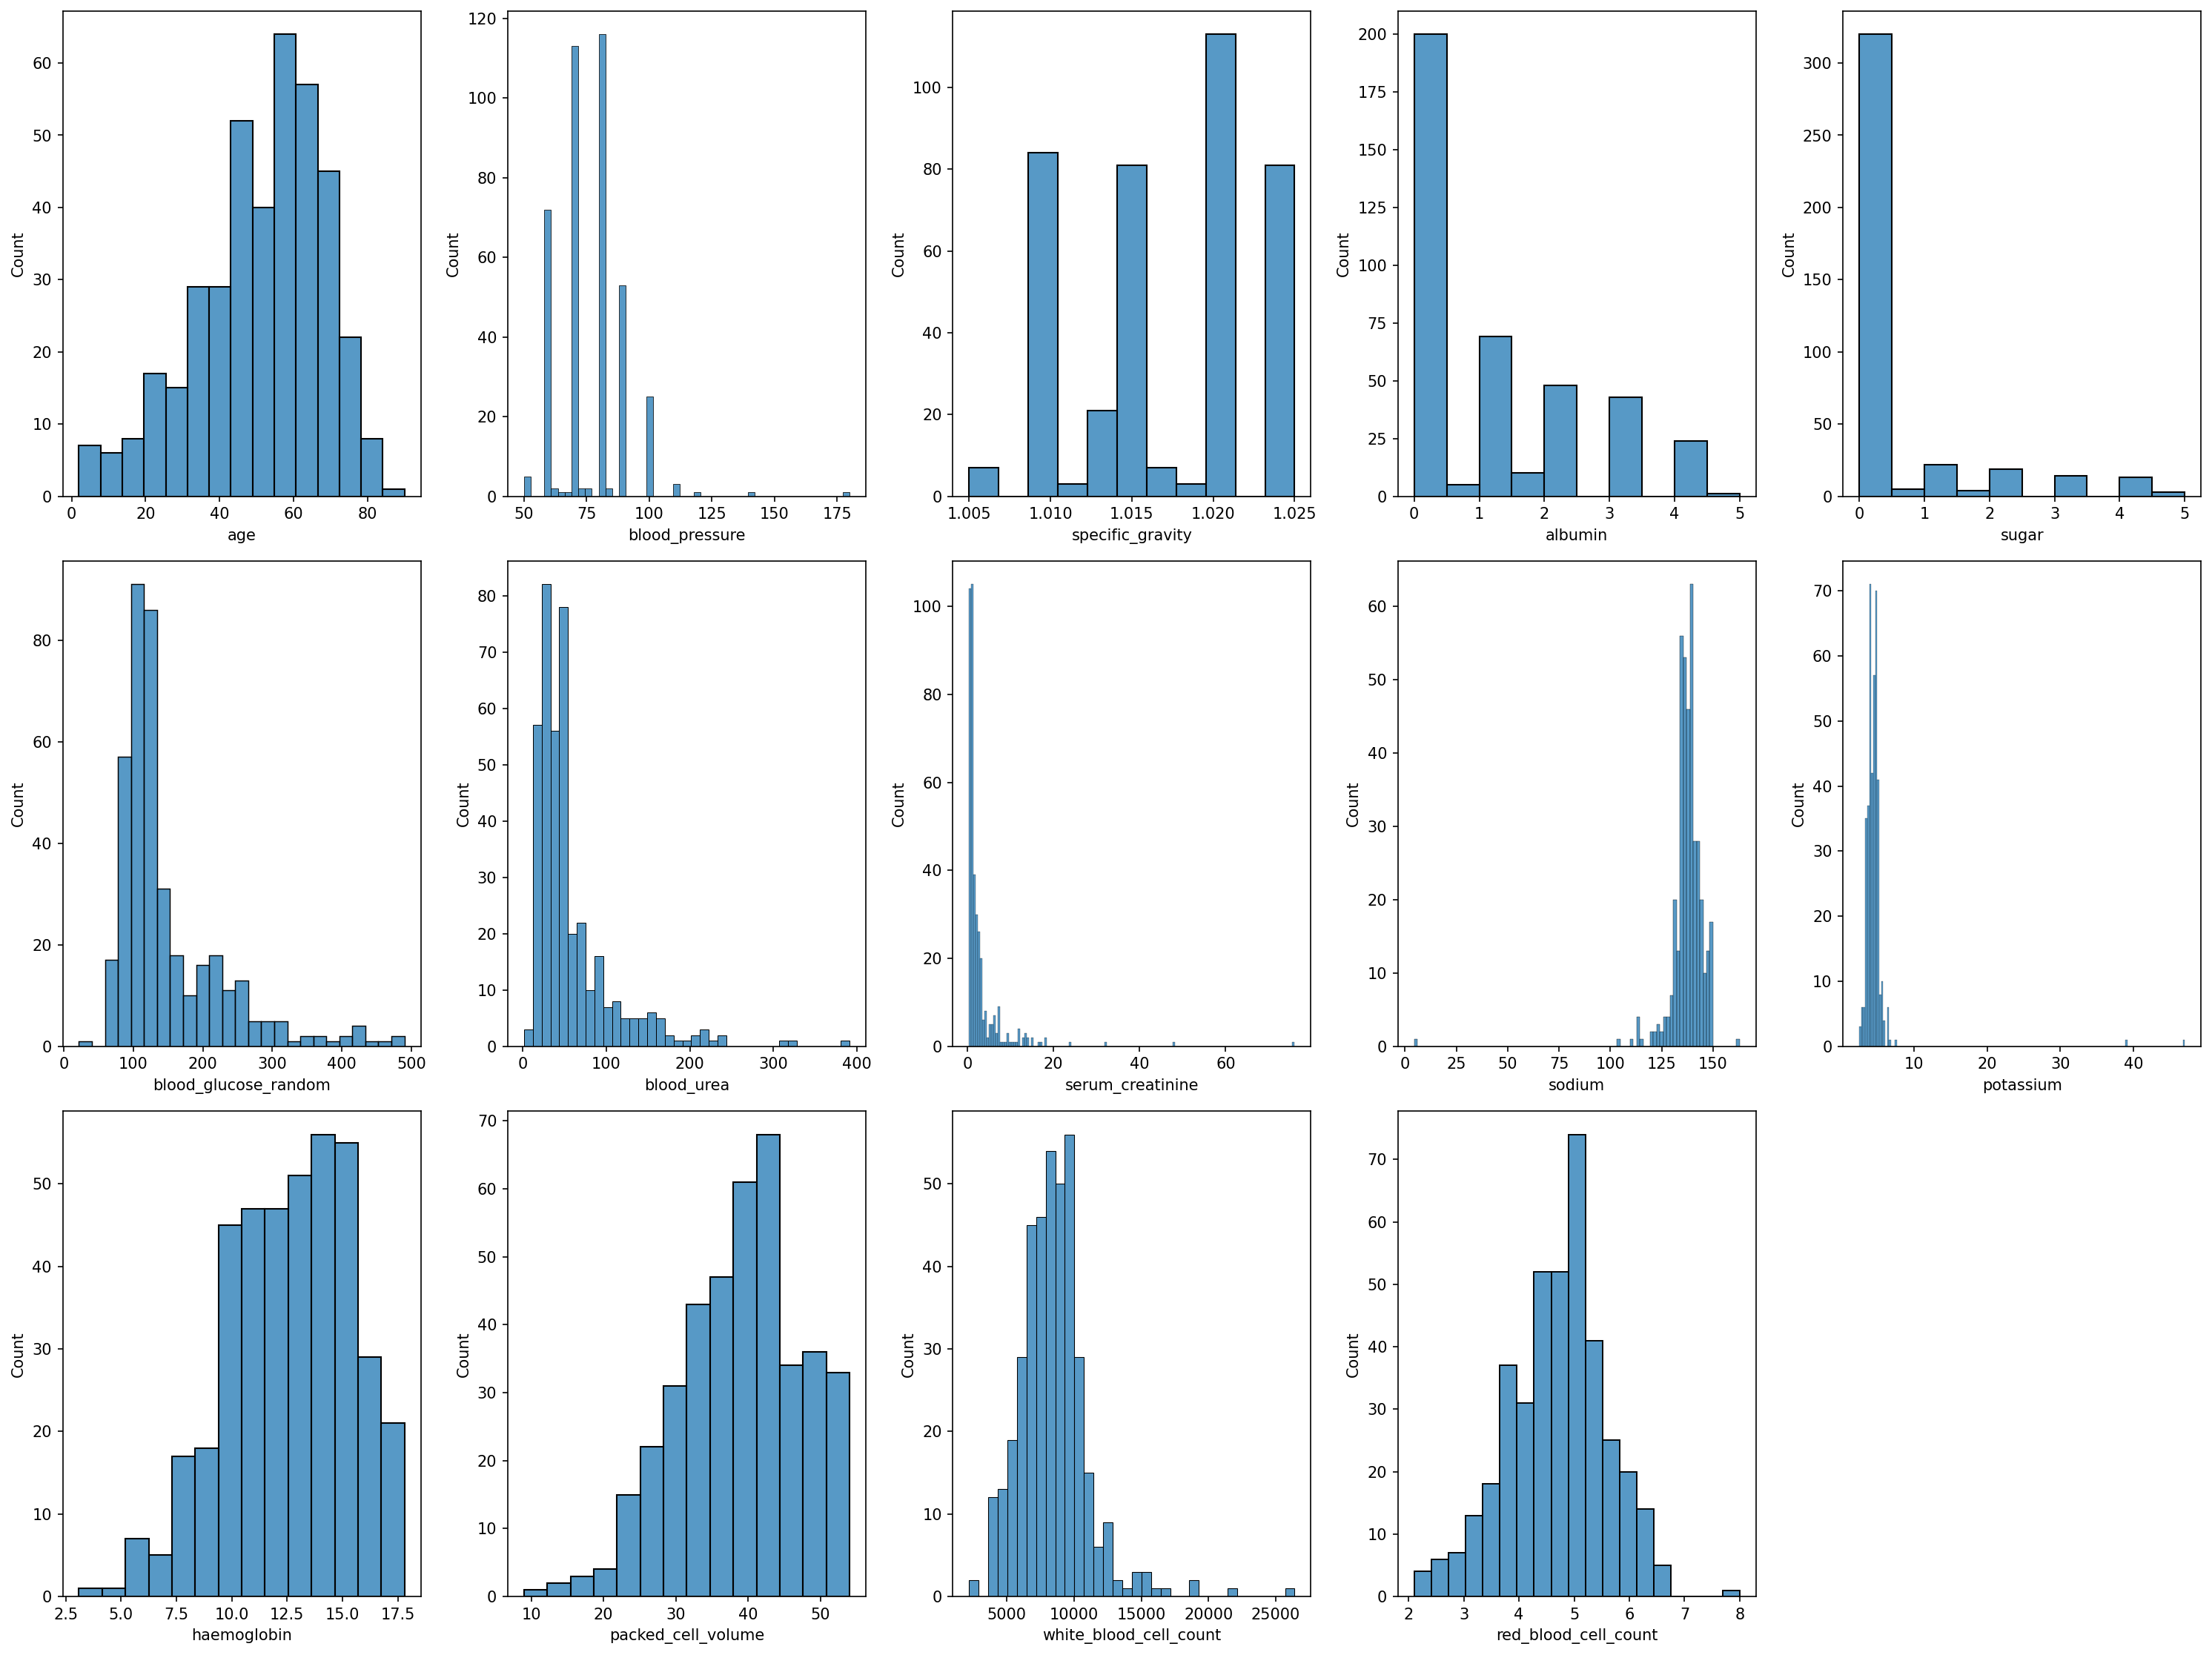
\includegraphics[width=0.92\textwidth]{01_distributions_numeriques.png}
\caption{Distributions des variables numériques du jeu CKD (après imputation).}
\label{fig:dist-num}
\end{figure}

La figure~\ref{fig:countplot} montre les effectifs des modalités pour les variables catégorielles (avant encodage). Cela permet de vérifier l'équilibre relatif des catégories et d'identifier d'éventuelles modalités rares.

\begin{figure}[H]
\centering
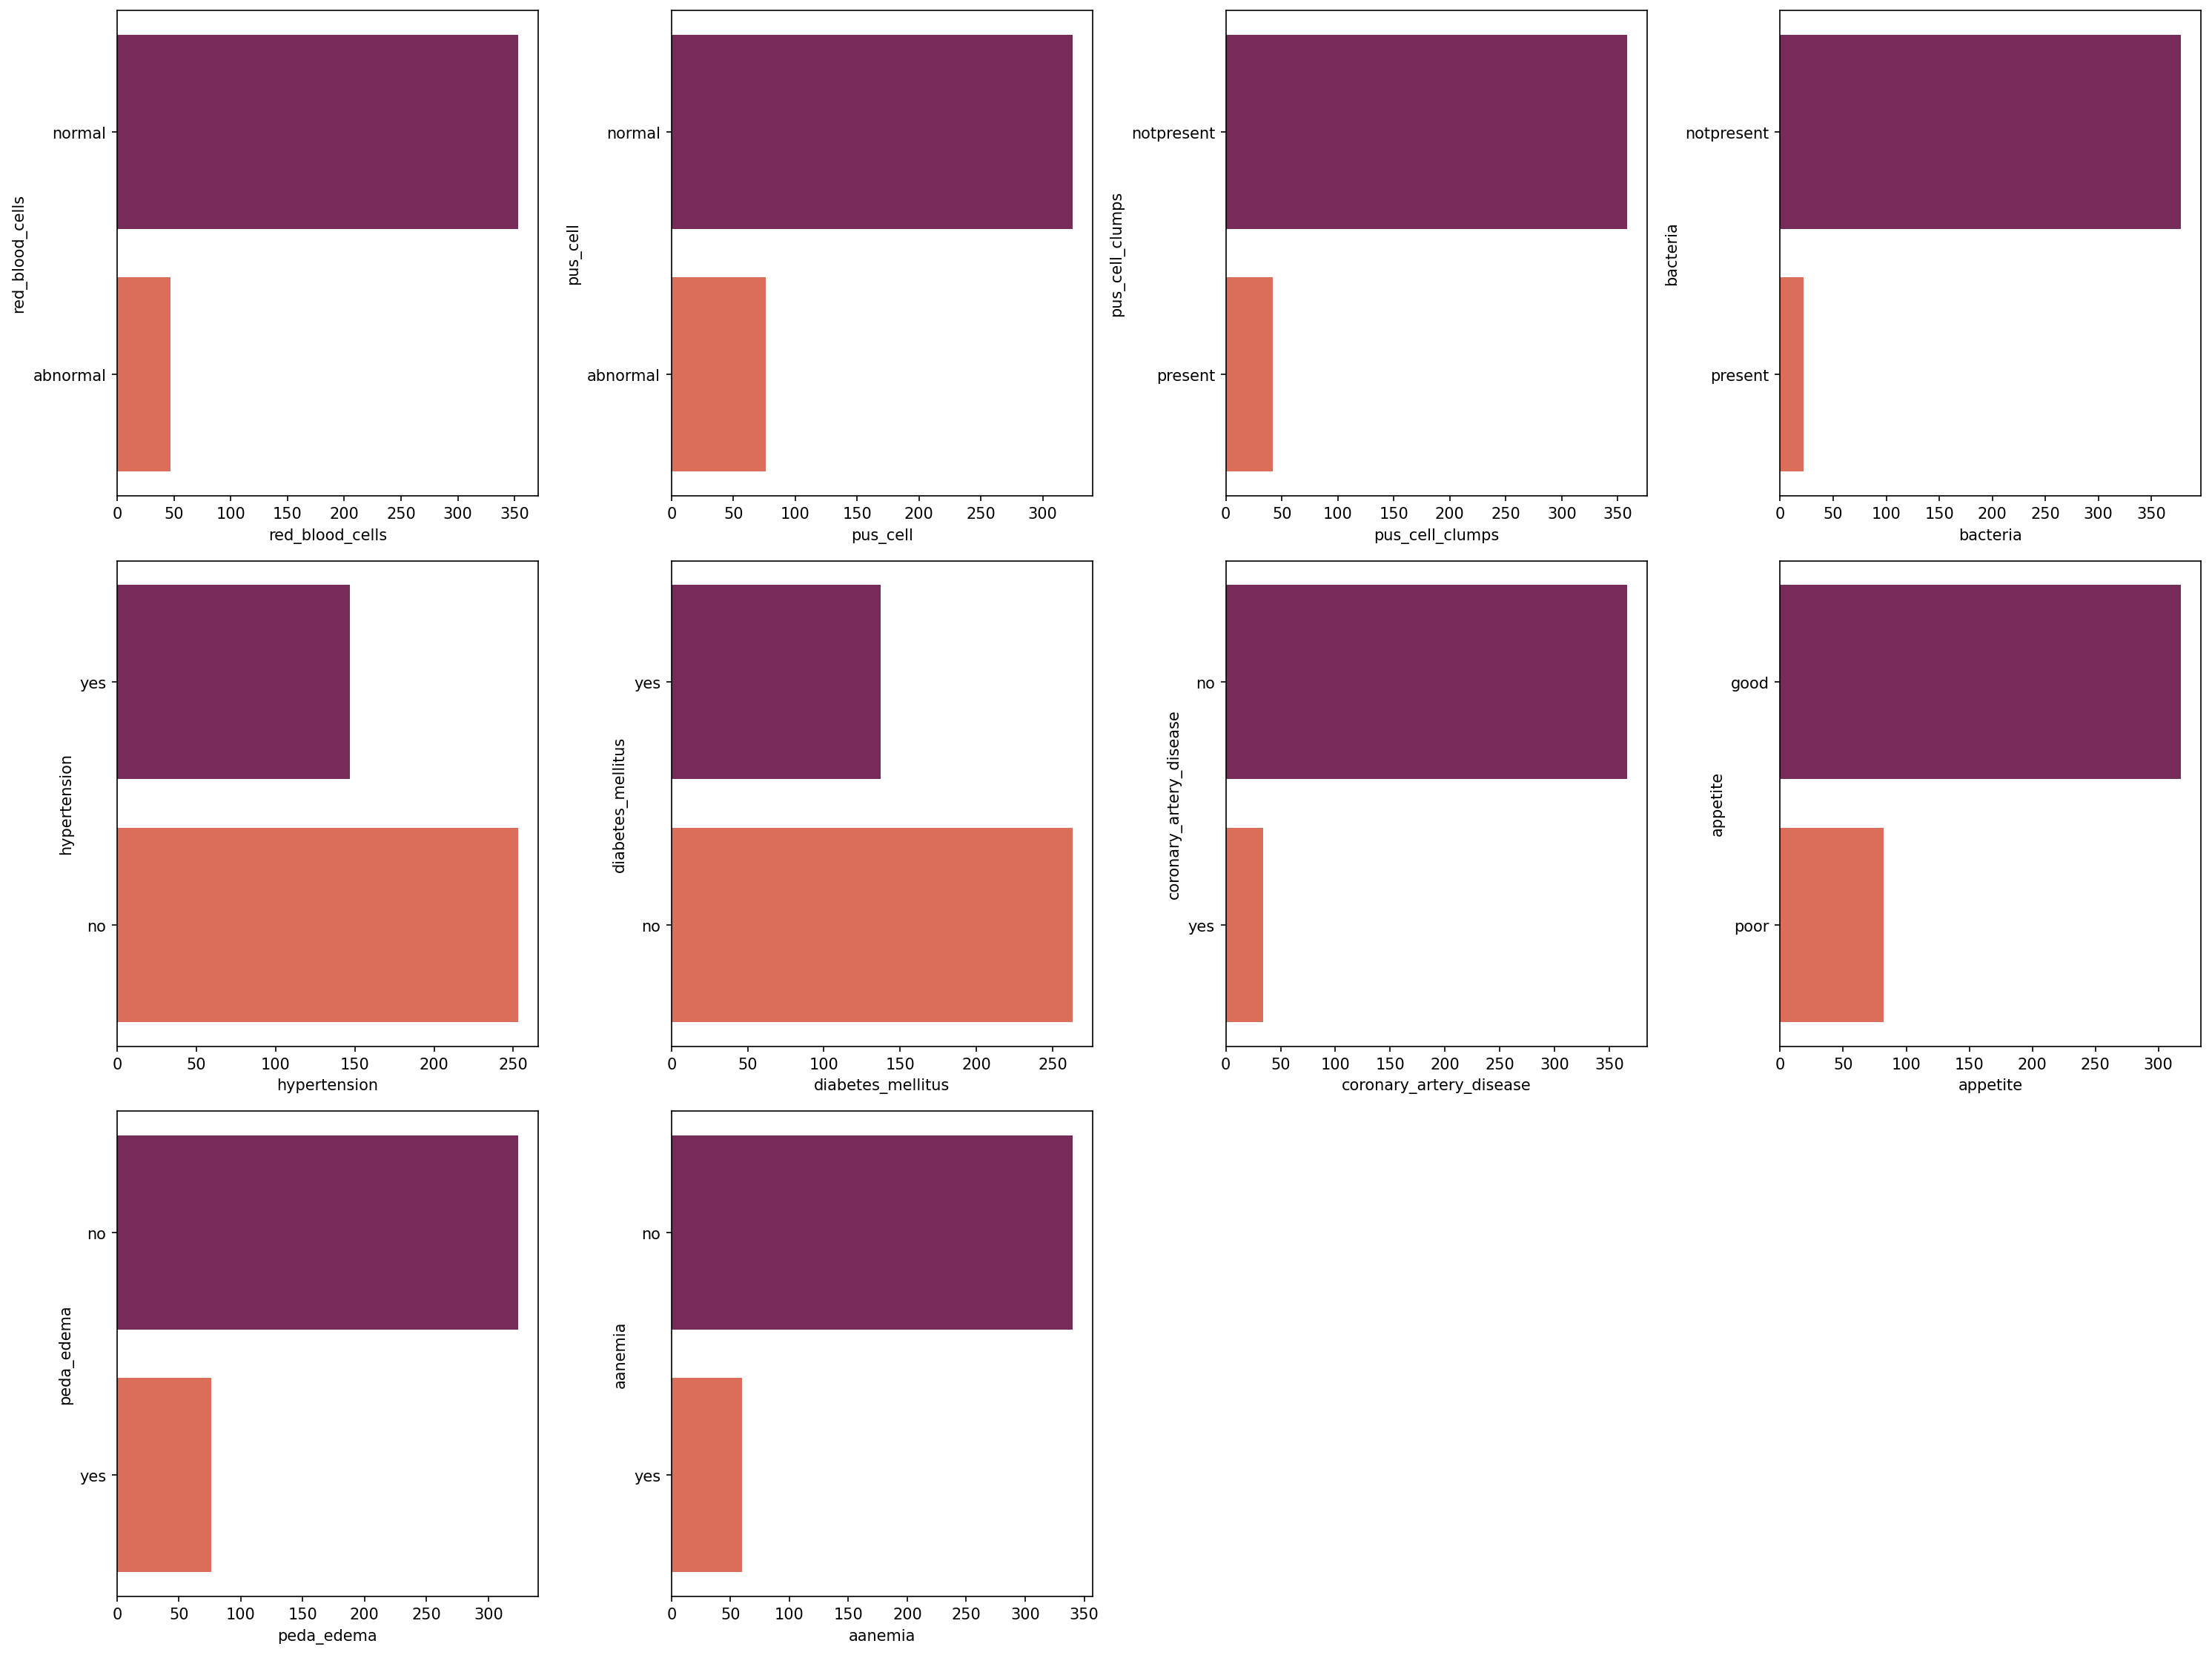
\includegraphics[width=0.88\textwidth]{02_categories_countplot.png}
\caption{Effectifs des variables catégorielles (avant encodage).}
\label{fig:countplot}
\end{figure}

La figure~\ref{fig:heatmap} présente la matrice de corrélation. Les variables déjà encodées sont incluses ; on peut repérer les paires d'attributs fortement corrélés (ex.\ hémoglobine et volume cellulaire), utiles pour l'interprétation des modèles.

\begin{figure}[H]
\centering
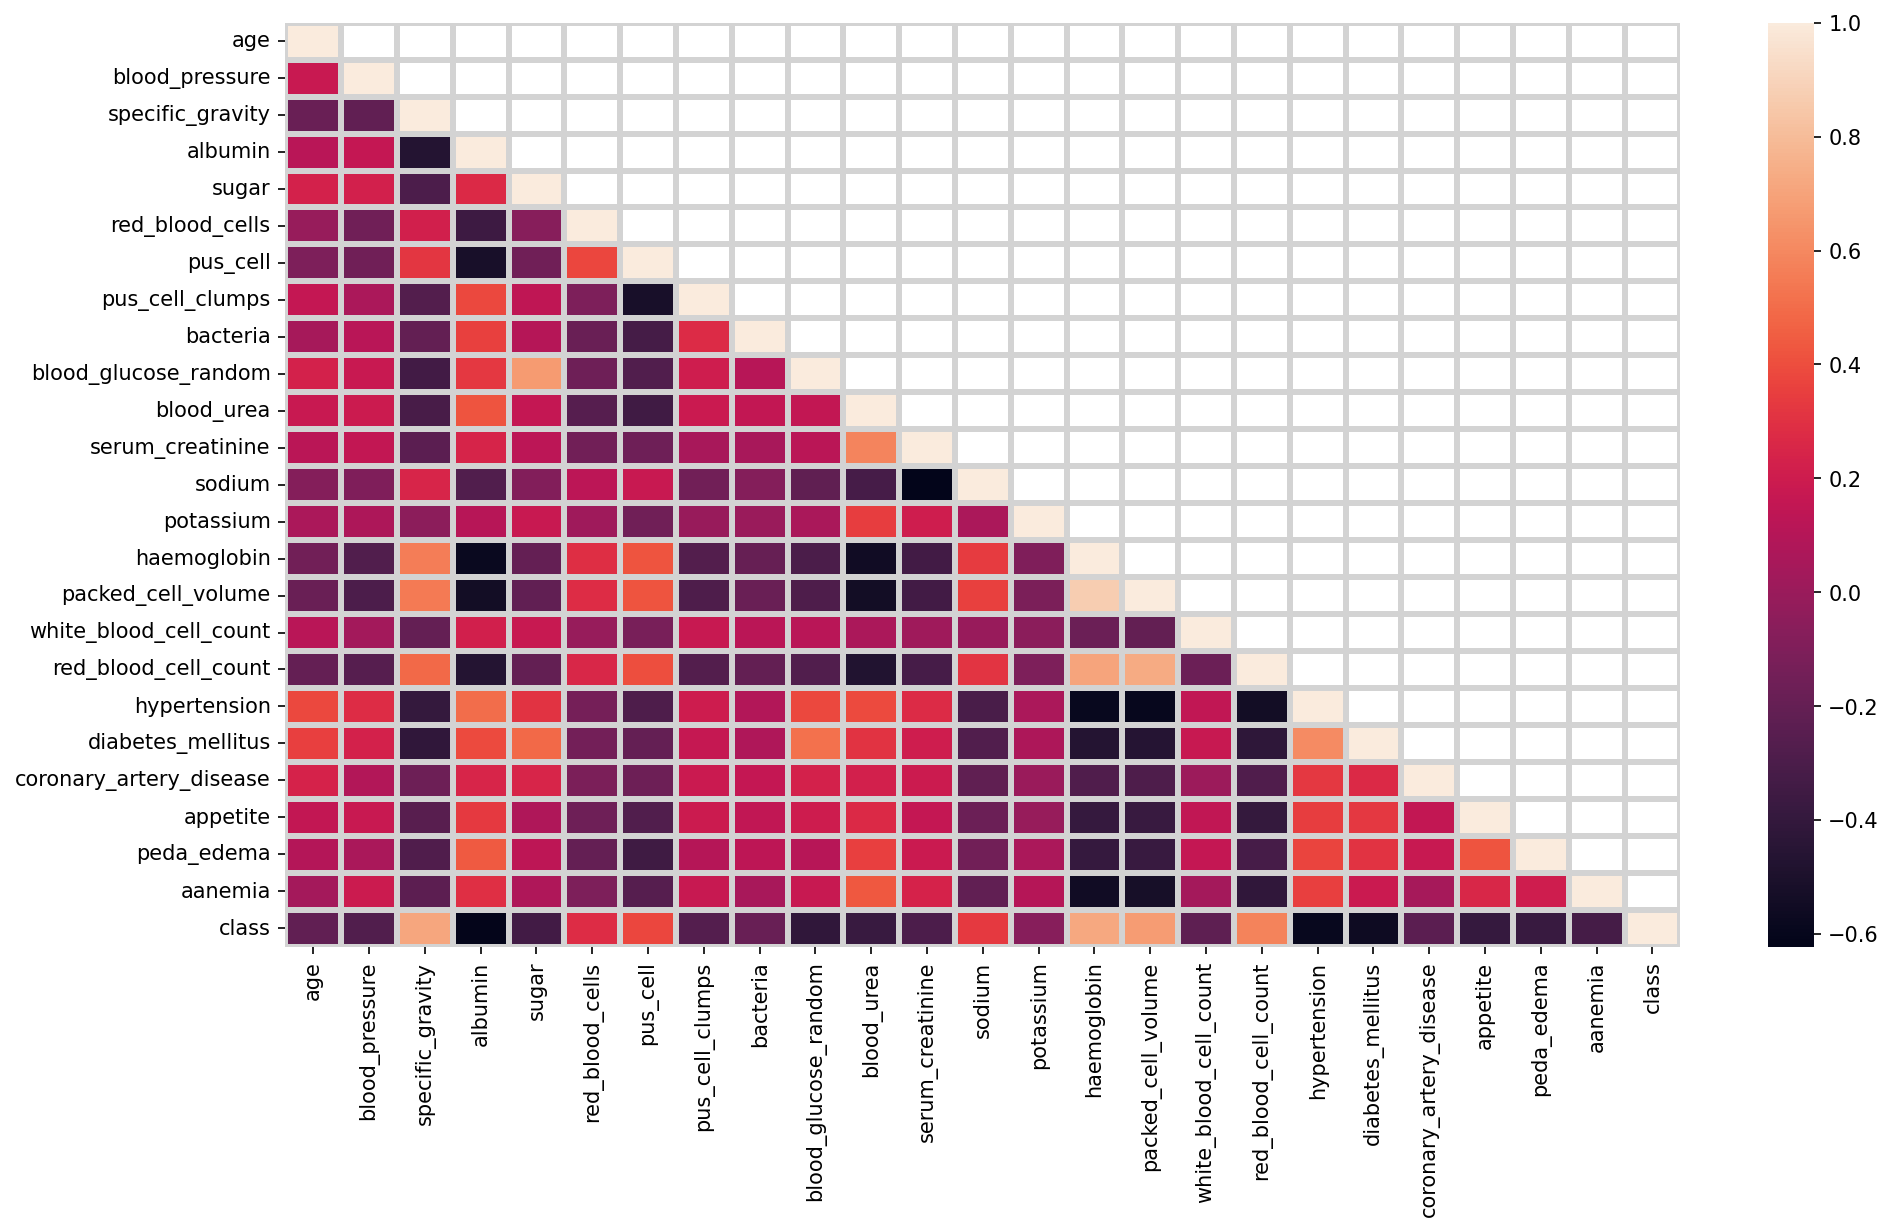
\includegraphics[width=0.90\textwidth]{03_heatmap_corr.png}
\caption{Matrice de corrélation (triangle inférieur) entre toutes les variables du jeu CKD.}
\label{fig:heatmap}
\end{figure}

\subsection{Découpage et équilibrage}

Le jeu préparé est divisé en ensembles d'entraînement et de test par \textbf{découpage stratifié} (\%~70 / 30) pour conserver les proportions de classes. La classe CKD étant souvent déséquilibrée, un rééquilibrage est appliqué sur l'ensemble d'entraînement uniquement avec \textbf{SMOTE} (technique de surotéchantillonnage de la minorité synthétique), avec $k = 3$ voisins, afin d'obtenir des effectifs de classes plus proches. Enfin, les variables numériques sont mises à l'échelle avec un \textbf{StandardScaler} (moyenne 0, écart-type 1), ajusté sur l'ensemble d'entraînement (après SMOTE) et appliqué aux données d'entraînement et de test. Les matrices ainsi obtenues (\texttt{X\_train\_scaled}, \texttt{X\_test\_scaled}) et les étiquettes associées sont utilisées dans les sections suivantes pour la régression logistique, l'arbre de décision, le SVM, LIME et SHAP.

\begin{lstlisting}[style=reportPython]
X_train, X_test, y_train, y_test = train_test_split(
    X, y, test_size=0.30, stratify=y, random_state=RANDOM_STATE)
smote = SMOTE(random_state=RANDOM_STATE, k_neighbors=3)
X_train_smote, y_train_smote = smote.fit_resample(X_train, y_train)
scaler = StandardScaler()
X_train_scaled = pd.DataFrame(scaler.fit_transform(X_train_smote), columns=feature_names)
X_test_scaled = pd.DataFrame(scaler.transform(X_test), columns=feature_names, index=X_test.index)
\end{lstlisting}

% Partie 2 : Explicabilité
\newpage
\section{Interprétabilité Intrinsèque desModèles }
\section{Explicabilité Post-Hoc des Modèles simples et Opaques }
% Partie 3 : Combinaison et explicabilité
\newpage
\section{Explicabilité des modèles de combinaison (bagging et boosting)}
\label{sec:cas3}

Les données utilisées sont celles préparées aux sections précédentes (jeu UCI maladie rénale chronique, CKD). On vise à illustrer l'explicabilité de deux modèles d'ensemble : une \textbf{forêt aléatoire} (\emph{Random Forest}, RF) et un modèle à \textbf{gradient boosting} (\emph{XGBoost}, XGB). Plusieurs techniques complémentaires sont appliquées —~TreeSHAP, distillation de connaissances, analyse des interactions SHAP~— pour fournir une vue locale, globale et auditables des prédictions.

\subsection{Modèles construits}
\label{ssec:cas3-modeles}

Deux modèles sont entraînés sur un jeu d'entraînement représentant 80\,\% des données (stratifié sur la variable cible), le reste étant réservé à l'évaluation et à l'explicabilité.

\begin{lstlisting}[style=reportPython]
from sklearn.ensemble import RandomForestClassifier
from xgboost import XGBClassifier
from sklearn.model_selection import train_test_split

X_train, X_test, y_train, y_test = train_test_split(
    X, y, test_size=0.20, random_state=42, stratify=y)

rf = RandomForestClassifier(n_estimators=100, random_state=42)
rf.fit(X_train, y_train)

xgb = XGBClassifier(n_estimators=100, use_label_encoder=False,
                     eval_metric='logloss', random_state=42)
xgb.fit(X_train, y_train)
\end{lstlisting}

Les deux modèles obtiennent des performances très élevées sur le jeu de test (exactitude supérieure à 98\,\%), cohérent avec la littérature. L'objet ici n'est pas de comparer les performances mais d'analyser la \textbf{transparence} de ces modèles au moyen de techniques d'explicabilité.

\subsection{TreeSHAP appliqué à la forêt aléatoire}
\label{ssec:cas3-treeshap}

\paragraph{Principe et mise en œuvre.}
TreeSHAP \cite{lundberg2020local} est une implémentation efficace des valeurs de Shapley pour les modèles arborescents : elle permet de calculer exactement, en temps polynomial, la contribution marginale de chaque variable à chaque prédiction. Un explicateur \texttt{TreeExplainer} est construit sur la forêt ; les valeurs SHAP sont calculées sur l'ensemble de test. La figure~\ref{fig:shap-rf-summary} présente le résumé agrégé (beeswarm) : chaque point est une observation, la couleur encode la valeur de la variable (rouge = élevée, bleu = faible), l'axe horizontal la contribution SHAP à la prédiction.

\begin{lstlisting}[style=reportPython]
import shap

explainer_rf = shap.TreeExplainer(rf)
shap_values_rf = explainer_rf.shap_values(X_test)

shap.summary_plot(shap_values_rf[1], X_test,
                  feature_names=feature_names, show=False)
plt.savefig('shap_rf_summary.png', bbox_inches='tight', dpi=150)
plt.close()
\end{lstlisting}

\begin{figure}[H]
\centering
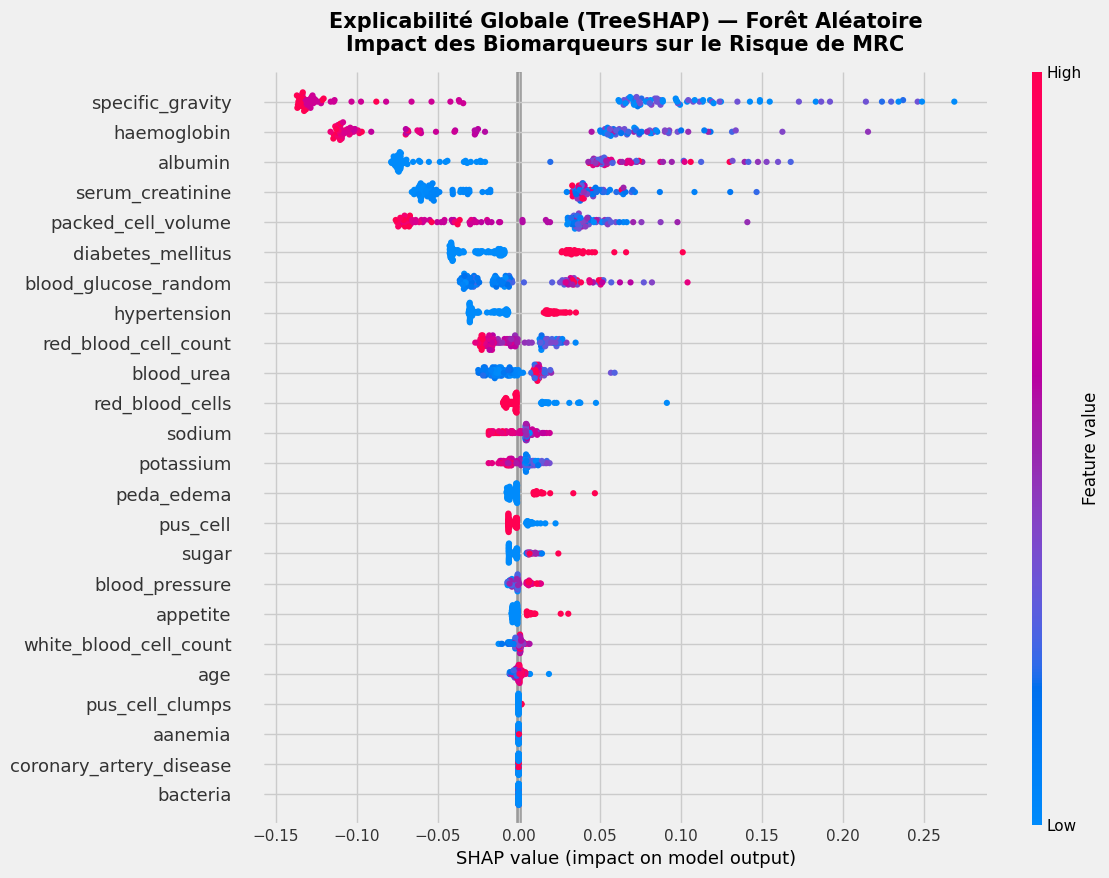
\includegraphics[width=0.95\textwidth]{cas_3/images/output1.png}
\caption{Valeurs SHAP agrégées sur le jeu de test — forêt aléatoire.}
\label{fig:shap-rf-summary}
\end{figure}

\paragraph{Interprétation.}
Le classement d'importance globale (Mean |SHAP|) place en tête \texttt{specific\_gravity} (22\,\%), \texttt{haemoglobin} (16\,\%), \texttt{albumin} (12{,}9\,\%), \texttt{serum\_creatinine} (9{,}5\,\%) et \texttt{packed\_cell\_volume} (9{,}2\,\%). Les corrélations de Spearman entre la valeur de chaque variable et sa valeur SHAP indiquent le sens de l'effet : négatif signifie que plus la variable augmente, plus le risque prédit baisse (ex.\ \texttt{haemoglobin} $r = -0{,}81$, \texttt{specific\_gravity} $r = -0{,}81$, \texttt{packed\_cell\_volume} $r = -0{,}80$) ; positif signifie que plus la variable augmente, plus le risque prédit augmente (ex.\ \texttt{serum\_creatinine} $r = +0{,}76$, \texttt{albumin} $r = +0{,}79$, \texttt{hypertension} $r = +0{,}82$). Un taux d'hémoglobine faible contribue ainsi positivement au risque CKD (anémie associée à l'insuffisance rénale) ; une créatinine sérique élevée augmente le risque prédit (réduction du débit de filtration glomérulaire). Le tableau~\ref{tab:shap-rf-top5} résume les statistiques descriptives des valeurs SHAP pour les cinq variables les plus importantes.

\begin{table}[H]
\centering
\caption{Statistiques descriptives des valeurs SHAP — Top 5 variables (forêt aléatoire).}
\label{tab:shap-rf-top5}
\small
\begin{tabular}{lrrrrr}
\hline
\textbf{Stat.} & \texttt{specific\_gravity} & \texttt{haemoglobin} & \texttt{albumin} & \texttt{serum\_creat.} & \texttt{packed\_cell\_vol.} \\
\hline
count & 120 & 120 & 120 & 120 & 120 \\
mean  & 0{,}014 & $-0{,}007$ & 0{,}006 & 0{,}003 & $-0{,}001$ \\
std   & 0{,}124 & 0{,}089 & 0{,}073 & 0{,}053 & 0{,}053 \\
min   & $-0{,}137$ & $-0{,}116$ & $-0{,}079$ & $-0{,}066$ & $-0{,}076$ \\
max   & 0{,}269 & 0{,}216 & 0{,}168 & 0{,}147 & 0{,}141 \\
\hline
\end{tabular}
\end{table}

\subsection{Distillation de connaissances}
\label{ssec:cas3-distillation}

\paragraph{Principe.}
La distillation consiste à entraîner un modèle simple et interprétable (ici un arbre de décision de profondeur 4) à reproduire les prédictions probabilistes (\emph{soft labels}) de la forêt aléatoire. On obtient une approximation globale du modèle opaque sous la forme d'un arbre lisible. Chaque feuille donne une probabilité CKD ; le seuil de décision clinique est 0{,}5. La figure~\ref{fig:distillation} montre la structure de l'arbre distillé.

\begin{lstlisting}[style=reportPython]
from sklearn.tree import DecisionTreeClassifier, export_text

soft_labels = rf.predict_proba(X_train)[:, 1]
student_tree = DecisionTreeClassifier(max_depth=4, random_state=42)
student_tree.fit(X_train, (soft_labels >= 0.5).astype(int))
tree_rules_text = export_text(student_tree, feature_names=list(X_train.columns))
\end{lstlisting}

La structure de l'arbre (pseudo-code clinique) est la suivante. La racine sépare sur \texttt{specific\_gravity} $\leq 1{,}02$ ; les nœuds suivants font intervenir \texttt{haemoglobin}, \texttt{packed\_cell\_volume}, \texttt{albumin}, \texttt{diabetes\_mellitus}, \texttt{hypertension}, \texttt{blood\_glucose\_random} et \texttt{sodium}. Les feuilles donnent des valeurs (probabilités) entre 0{,}02 et 1{,}00 ; une probabilité $\geq 0{,}5$ conduit à la prédiction CKD.

\begin{figure}[H]
\centering
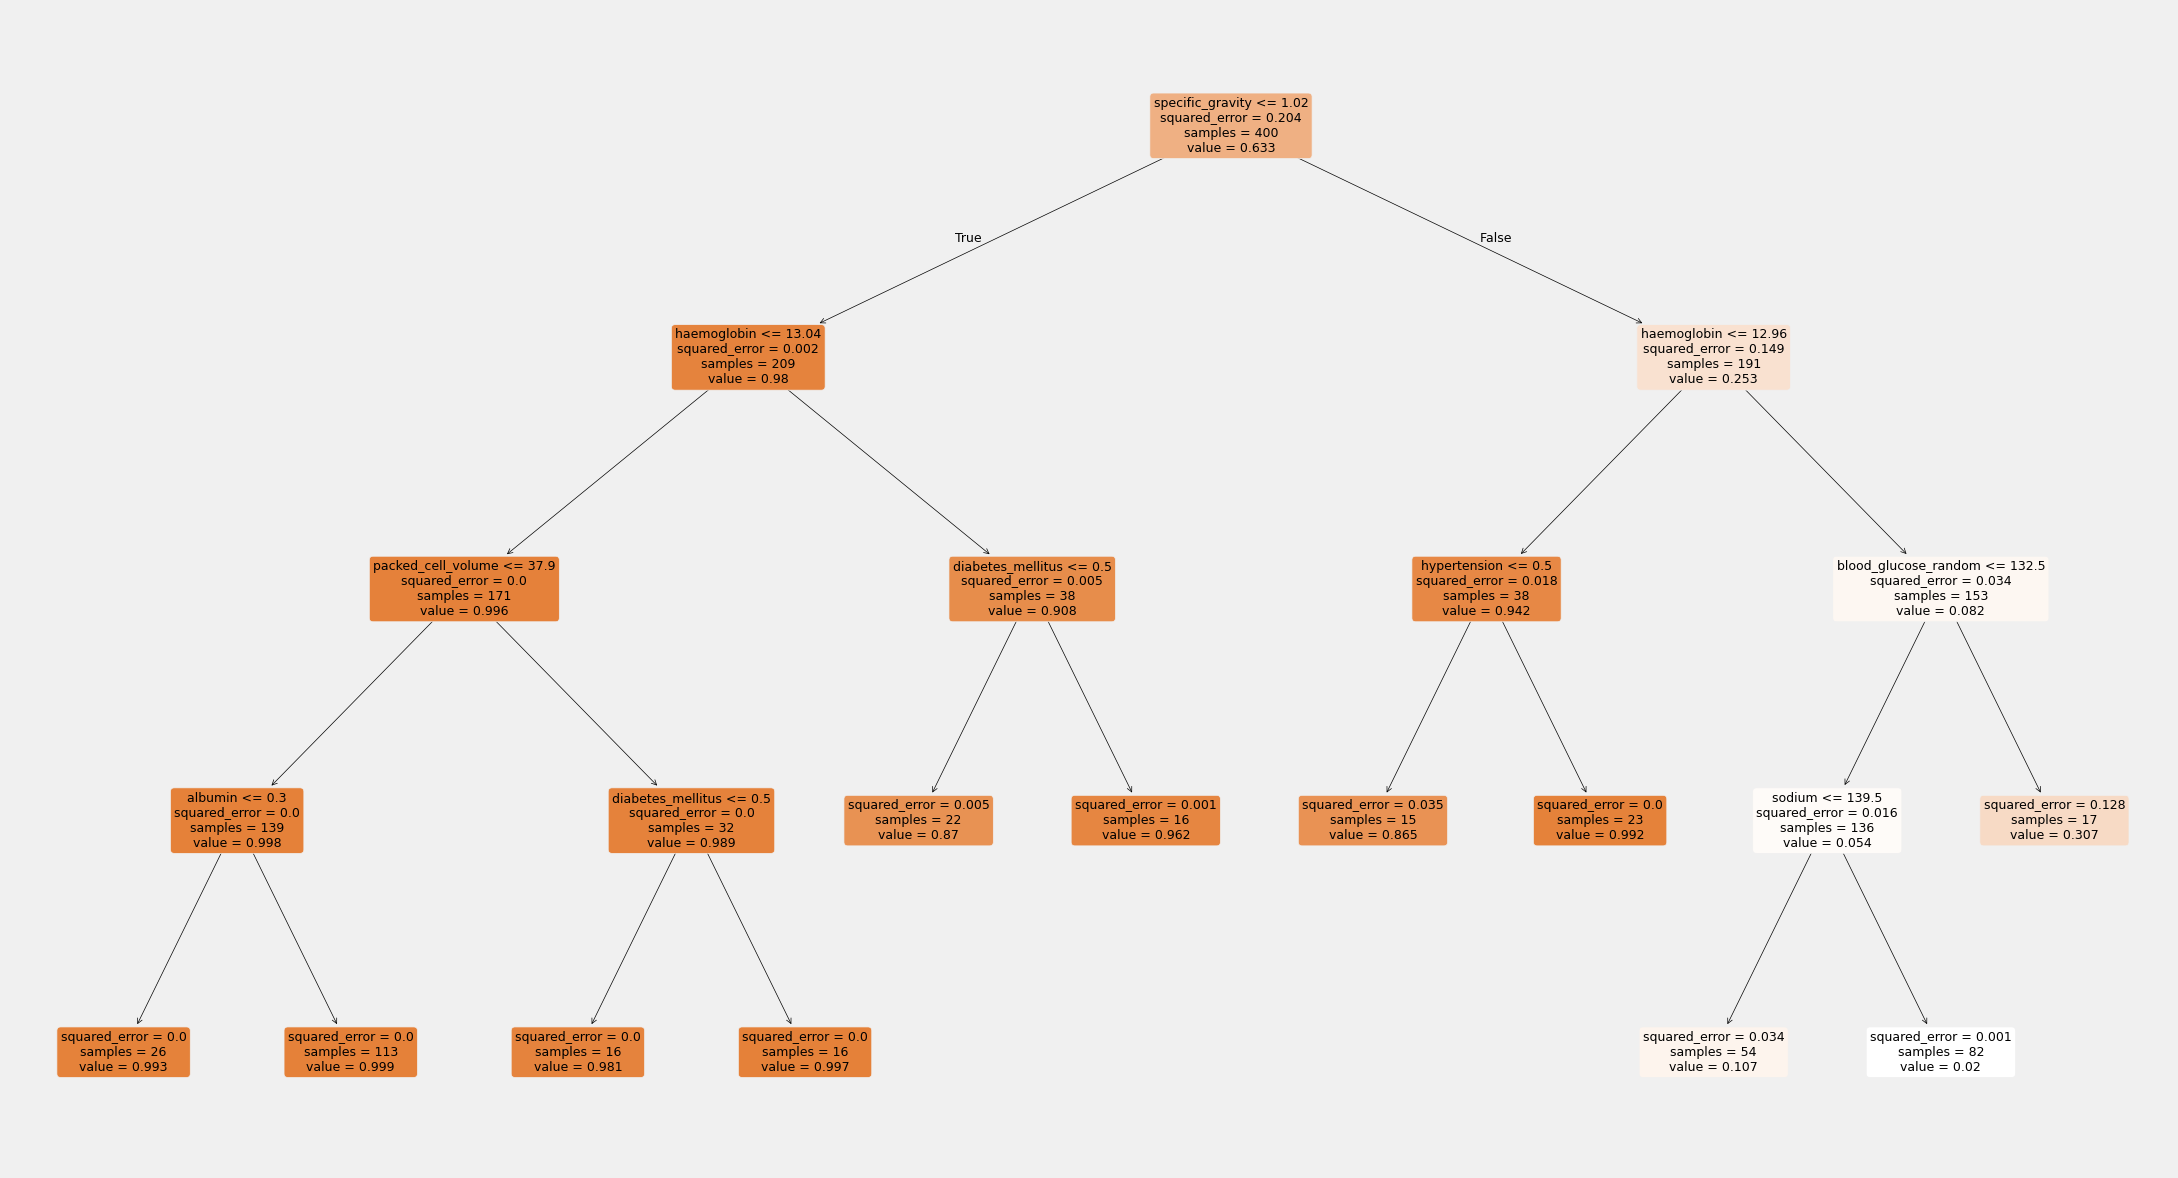
\includegraphics[width=0.95\textwidth]{cas_3/images/output2.png}
\caption{Arbre de décision distillé depuis la forêt aléatoire (profondeur max.\,4).}
\label{fig:distillation}
\end{figure}

\paragraph{Importance des variables (Gini) et interprétation.}
L'importance des variables dans l'arbre distillé (impureté de Gini) est dominée par \texttt{specific\_gravity} (68{,}6\,\%) et \texttt{haemoglobin} (29{,}6\,\%) ; viennent ensuite \texttt{blood\_glucose\_random}, \texttt{sodium}, \texttt{hypertension} et \texttt{diabetes\_mellitus} (tableau~\ref{tab:distill-gini}). La fidélité de l'arbre distillé (accord avec les prédictions de la RF sur le jeu de test) est supérieure à 96\,\% : le comportement global du modèle opaque est bien capturé par un arbre de profondeur 4. Cette hiérarchie (gravité spécifique et hémoglobine en tête) est \textbf{cohérente avec les valeurs SHAP} (section~\ref{ssec:cas3-treeshap}).

\begin{table}[H]
\centering
\caption{Importance des variables dans l'arbre distillé (Gini).}
\label{tab:distill-gini}
\small
\begin{tabular}{lc}
\hline
\textbf{Variable} & \textbf{Importance (\,\%)} \\
\hline
\texttt{specific\_gravity}  & 68{,}6 \\
\texttt{haemoglobin}         & 29{,}6 \\
\texttt{blood\_glucose\_random} & 1{,}3 \\
\texttt{sodium}              & 0{,}3 \\
\texttt{hypertension}        & 0{,}2 \\
\texttt{diabetes\_mellitus}  & 0{,}1 \\
\hline
\end{tabular}
\end{table}

\subsection{Interactions SHAP appliquées à XGBoost}
\label{ssec:cas3-shap-interactions}

\paragraph{Classement global et corrélations (XGBoost).}
Pour XGBoost, le classement d'importance globale (Mean |SHAP|) place en tête \texttt{haemoglobin} (19{,}3\,\%), \texttt{specific\_gravity} (18{,}9\,\%), \texttt{serum\_creatinine} (14\,\%), \texttt{albumin} (12{,}5\,\%) et \texttt{packed\_cell\_volume} (7{,}4\,\%). Les corrélations de Spearman (valeur de la variable $\leftrightarrow$ SHAP) indiquent le sens de l'effet : \texttt{haemoglobin} $r = +0{,}81$, \texttt{specific\_gravity} $r = +0{,}79$, \texttt{serum\_creatinine} $r = -0{,}76$, \texttt{albumin} $r = -0{,}80$, \texttt{blood\_glucose\_random} $r = -0{,}90$. Le tableau~\ref{tab:shap-xgb-top5} donne les statistiques descriptives des valeurs SHAP pour les cinq variables les plus importantes.

\begin{table}[H]
\centering
\caption{Statistiques descriptives des valeurs SHAP — Top 5 variables (XGBoost).}
\label{tab:shap-xgb-top5}
\small
\begin{tabular}{lrrrrr}
\hline
\textbf{Stat.} & \texttt{haemoglobin} & \texttt{specific\_gravity} & \texttt{serum\_creat.} & \texttt{albumin} & \texttt{packed\_cell\_vol.} \\
\hline
count & 120 & 120 & 120 & 120 & 120 \\
mean  & $-0{,}005$ & $-0{,}534$ & $-0{,}092$ & $-0{,}356$ & $-0{,}149$ \\
std   & 1{,}686 & 1{,}588 & 1{,}230 & 1{,}053 & 0{,}617 \\
min   & $-3{,}23$ & $-3{,}78$ & $-2{,}15$ & $-2{,}42$ & $-1{,}37$ \\
max   & 2{,}39 & 1{,}59 & 1{,}71 & 0{,}85 & 0{,}90 \\
\hline
\end{tabular}
\end{table}

\paragraph{Dependence plot et interaction Hémoglobine $\times$ Diabète.}
Les valeurs SHAP d'interaction généralisent les valeurs de Shapley au second ordre. Le graphique de dépendance représente, pour une variable donnée, sa contribution SHAP en fonction de sa valeur, avec une coloration par une seconde variable, ce qui révèle visuellement les interactions. La figure~\ref{fig:shap-dependence} illustre l'hémoglobine en fonction du statut diabétique.

\begin{lstlisting}[style=reportPython]
import shap

explainer_xgb = shap.TreeExplainer(xgb)
shap_values_xgb = explainer_xgb.shap_values(X_test)

shap.dependence_plot(
    "haemoglobin", shap_values_xgb, X_test_df,
    interaction_index="diabetes_mellitus",
    feature_names=feature_names, show=False)
plt.savefig('shap_xgb_dependence_hemo_dm.png',
            bbox_inches='tight', dpi=150)
plt.close()
\end{lstlisting}

Le tableau~\ref{tab:shap_interaction} donne la moyenne et l'écart-type des valeurs SHAP de l'hémoglobine selon le statut diabétique (jeu de test, XGBoost). La corrélation de Spearman entre le taux d'hémoglobine et sa valeur SHAP est $r = +0{,}860$ dans le groupe non diabétique et $r = +0{,}069$ dans le groupe diabétique.

\begin{table}[H]
\centering
\caption{Moyenne et écart-type des valeurs SHAP de l'hémoglobine selon le statut diabétique (jeu de test, XGBoost).}
\label{tab:shap_interaction}
\begin{tabular}{lccc}
\hline
\textbf{Groupe} & \textbf{Moyenne SHAP} & \textbf{Écart-type} & \textbf{Effectif} \\
\hline
Non diabétique (dm = 0) & $+0.5669$ & $1.6606$ & 85 \\
Diabétique (dm = 1)     & $-1.3931$ & $0.5789$ & 35 \\
\hline
\end{tabular}
\end{table}

\begin{figure}[H]
\centering
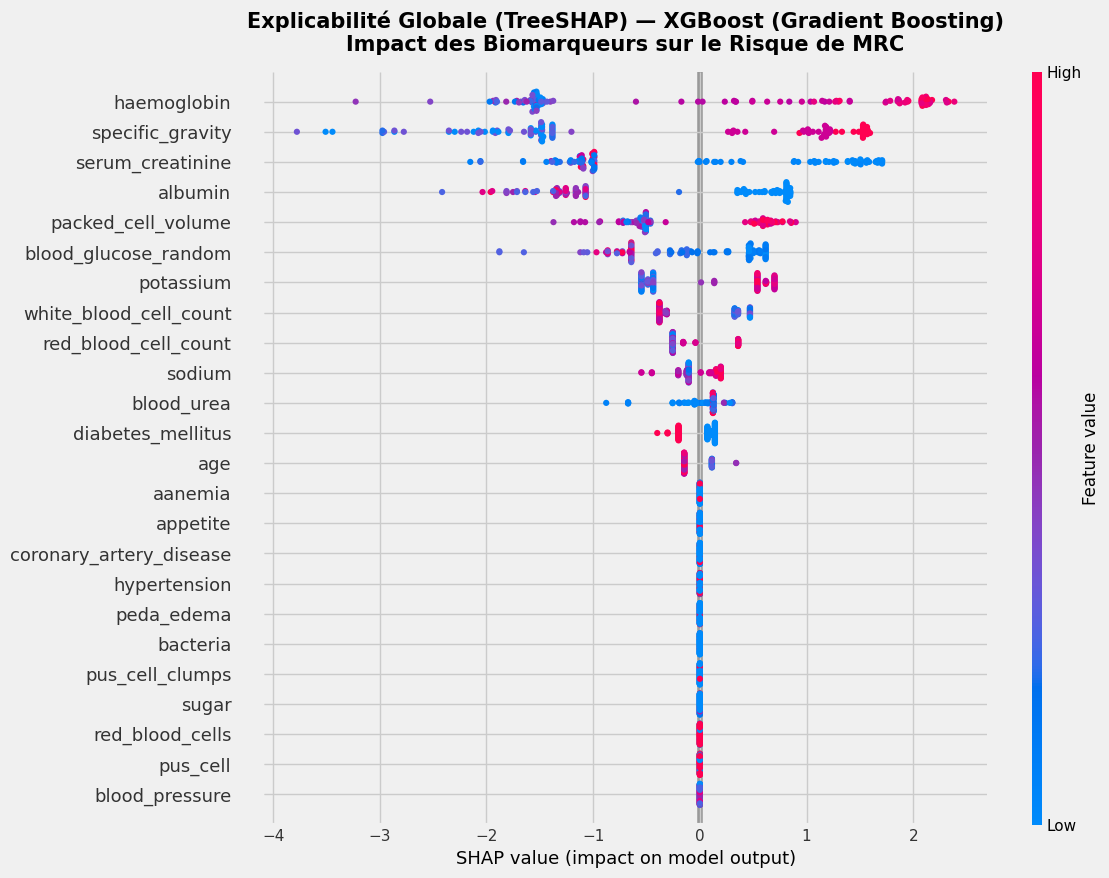
\includegraphics[width=0.95\textwidth]{cas_3/images/output3.png}
\caption{Graphique de dépendance SHAP (XGBoost). Axe des abscisses : taux d'hémoglobine (g/dL). Couleur : rouge = diabétique (dm = 1), bleu = non diabétique (dm = 0).}
\label{fig:shap-dependence}
\end{figure}

\paragraph{Interprétation.}
La moyenne des valeurs SHAP pour l'hémoglobine est $+0{,}57$ chez les non diabétiques (dm = 0) et $-1{,}39$ chez les diabétiques (dm = 1) (tableau~\ref{tab:shap_interaction}). La corrélation Hémoglobine $\leftrightarrow$ SHAP (hémoglobine) est $r = +0{,}86$ dans le groupe non diabétique et $r = +0{,}07$ dans le groupe diabétique : une corrélation négative signifierait que plus l'hémoglobine baisse, plus la contribution au risque CKD augmente ; ici, chez les diabétiques, l'hémoglobine perd sa valeur discriminante, le modèle s'appuyant davantage sur d'autres variables. Dans la plage intermédiaire (environ 10--12\,g/dL), les points rouges (diabétiques) se situent au-dessus des points bleus : pour un même degré d'anémie modérée, un patient diabétique reçoit une contribution SHAP plus élevée (risque plus grand). Ceci reflète l'interaction biologique de la \textbf{néphropathie diabétique}. L'analyse SHAP permet ainsi de détecter des \textbf{interactions non linéaires} que les méthodes d'importance globale ne révèlent pas.

\paragraph{Valeurs d'interaction Shapley-Taylor et graphique clinique.}
Pour aller au-delà des contributions marginales, on calcule le \textbf{tenseur d'interactions SHAP} (décomposition de type Shapley-Taylor) via \texttt{shap\_interaction\_values} : pour chaque observation, on obtient une matrice $p \times p$ qui décompose les contributions au second ordre (interaction entre paires de variables). La forme du tenseur est $(n, p, p)$. Le graphique de dépendance (hémoglobine en abscisse, valeur SHAP en ordonnée, coloration par \texttt{diabetes\_mellitus} avec nuancier coolwarm) est ensuite produit à partir des valeurs SHAP standard ; un titre explicite met en avant l'«~interaction clinique : Hémoglobine $\times$ Diabète sucré~» et l'effet non linéaire et modulé de l'hémoglobine sur le risque de CKD. La figure~\ref{fig:shap-interaction-clinique} présente ce graphique.

\begin{lstlisting}[style=reportPython]
shap_interaction_values = explainer_xgb.shap_interaction_values(X_test)

shap_vals_xgb = np.asarray(shap_values_xgb, dtype=np.float64)
X_test_vals = np.asarray(X_test, dtype=np.float64)
shap.dependence_plot(
    "haemoglobin", shap_vals_xgb, X_test_vals,
    interaction_index="diabetes_mellitus",
    feature_names=list(X_test.columns), show=False,
    cmap=plt.get_cmap("coolwarm"))
ax = plt.gca()
ax.set_title(
    "Interaction Clinique : Hemoglobine x Diabete Sucre\n"
    "Effet non lineaire et module (XGBoost)", fontsize=14)
ax.set_xlabel("Taux d'Hemoglobine (g/dL)", fontsize=12)
ax.set_ylabel("Valeur SHAP (contribution au log-odds CKD)", fontsize=11)
plt.tight_layout()
plt.savefig('output4.png', bbox_inches='tight', dpi=150)
\end{lstlisting}

\begin{figure}[H]
\centering
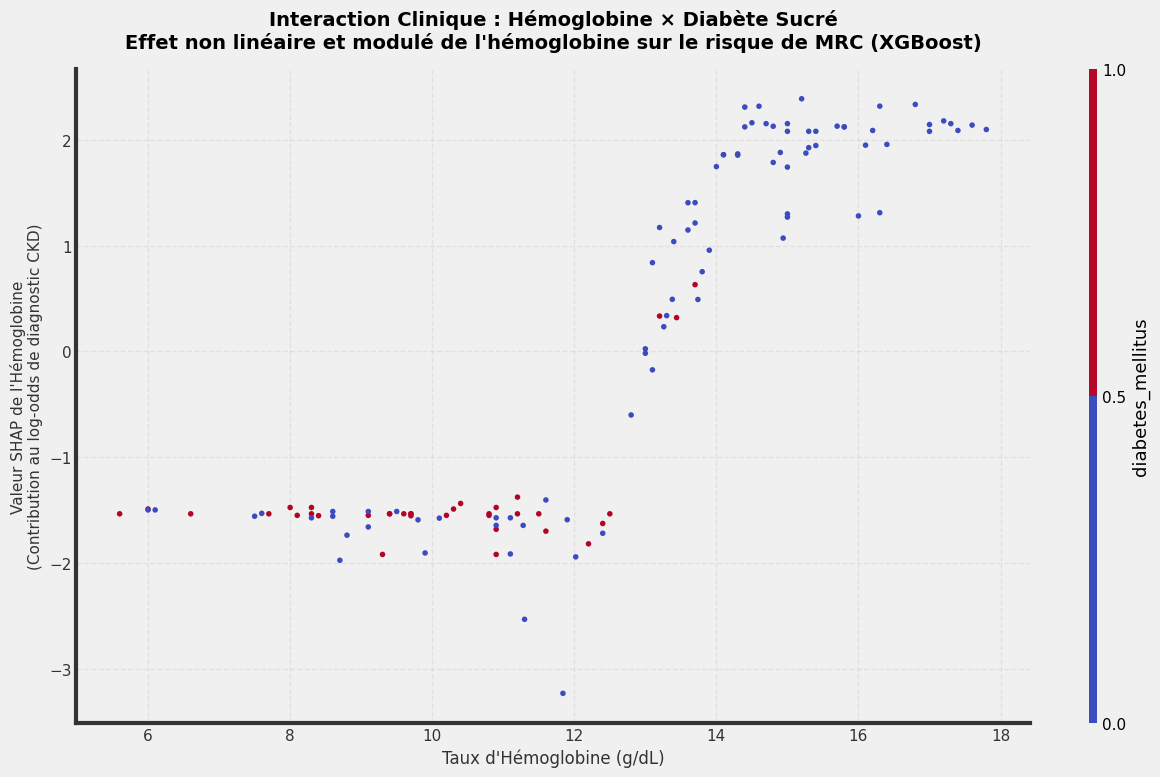
\includegraphics[width=0.95\textwidth]{cas_3/images/output4.png}
\caption{Interaction clinique : Hémoglobine $\times$ Diabète sucré — effet non linéaire et modulé de l'hémoglobine sur le risque de CKD (XGBoost). Axe des abscisses : taux d'hémoglobine (g/dL). Couleur : \texttt{diabetes\_mellitus} (bleu = faible, rouge = élevé).}
\label{fig:shap-interaction-clinique}
\end{figure}

Ce graphique résume visuellement comment le statut diabétique module la relation entre le taux d'hémoglobine et sa contribution au log-odds de diagnostic CKD : en zone intermédiaire (environ 12--14\,g/dL), la pente et le niveau des valeurs SHAP diffèrent selon que le patient est diabétique ou non, ce qui illustre la \textbf{néphropathie diabétique} sans qu'elle soit encodée explicitement dans le modèle.

\subsection{Tableau de gouvernance}
\label{ssec:cas3-gouvernance}

En vue d'auditabilité et de conformité (ex.\ cadre de l'IA Act européen), les propriétés des deux modèles sont synthétisées dans le tableau~\ref{tab:gouvernance}.

\begin{table}[H]
\centering
\caption{Tableau de gouvernance — comparaison des propriétés d'explicabilité.}
\label{tab:gouvernance}
\begin{tabular}{lcc}
\hline
\textbf{Critère} & \textbf{Random Forest} & \textbf{XGBoost} \\
\hline
Explicabilité locale (SHAP)      & Oui (TreeSHAP)    & Oui (TreeSHAP)    \\
Distillation possible            & Oui (fidélité > 96\,\%) & Oui          \\
Interactions détectables (SHAP)  & Oui               & Oui (plus stable) \\
Stabilité des explications       & Modérée           & Élevée            \\
Complexité du modèle             & Modérée           & Élevée            \\
\hline
\end{tabular}
\end{table}

XGBoost présente des valeurs SHAP plus stables grâce à la régularisation ($L_1$, $L_2$) intégrée.

\subsection{Synthèse}

Les techniques d'explicabilité appliquées aux modèles d'ensemble (RF, XGBoost) sur le jeu CKD donnent des résultats cohérents et cliniquement pertinents : la gravité spécifique (\texttt{specific\_gravity}), l'hémoglobine, l'albumine, la créatinine sérique et le volume globulaire apparaissent comme les variables les plus contributives (SHAP global, importance Gini dans l'arbre distillé). La distillation valide qu'un arbre de profondeur 4 approxime bien le comportement de la forêt avec une fidélité élevée, la racine et l'importance Gini mettant en avant la gravité spécifique et l'hémoglobine. L'analyse d'interaction SHAP (moyenne SHAP par groupe diabète, corrélations $r = +0{,}86$ / $r = +0{,}07$) révèle que le diabète est un modificateur d'effet fort sur la relation hémoglobine--risque CKD, en accord avec la néphropathie diabétique. La combinaison d'explications locales (SHAP) et de modèles distillés couvre un large besoin en explicabilité pour les applications médicales.


% Conclusion
\newpage
\section{Approches Avancées d'Explicabilité}

\newpage
\renewcommand{\refname}{Références}
\bibliographystyle{plain}
\bibliography{bibliographie}

\end{document}
